\documentclass[12 pt]{article}
\usepackage[utf8]{inputenc}
\usepackage{matlab-prettifier}
\usepackage[portuguese]{babel}
\usepackage{indentfirst}
\usepackage{graphicx}
\usepackage{float}
\usepackage{subcaption}
\usepackage[font=small,labelfont=bf]{caption}
\definecolor{mygreen}{RGB}{28,172,0} % color values Red, Green, Blue
\definecolor{myyellow}{rgb}{1.0, 1.0, 0.8}
\usepackage{mathtools}
\usepackage{multirow}
\usepackage{comment}
\usepackage{xcolor}
\usepackage{colortbl}
\usepackage[normalem]{ulem}               % to striketrhourhg text
\usepackage{amsmath}
\usepackage{amsfonts}
\newcommand\redout{\bgroup\markoverwith
{\textcolor{red}{\rule[0.5ex]{2pt}{0.8pt}}}\ULon}
\renewcommand{\lstlistingname}{Código}% Listing -> Algorithm
\renewcommand{\lstlistlistingname}{Lista de \lstlistingname s}% List of Listings -> List of Algorithms

\usepackage[top=3cm,left=2cm,bottom=2cm, right=2cm]{geometry}

% Configuração para destacar a sintaxe do Python
\lstset{ 
    language=Python,                     % A linguagem do código
    backgroundcolor=\color{myyellow}, % A cor do fundo 
    basicstyle=\ttfamily\footnotesize,   % O estilo do texto básico
    keywordstyle=\color{blue},           % Cor das palavras-chave
    stringstyle=\color{red},             % Cor das strings
    commentstyle=\color{mygreen},          % Cor dos comentários
    numbers=left,                        % Números das linhas à esquerda
    numberstyle=\tiny\color{gray},       % Estilo dos números das linhas
    stepnumber=1,                        % Número de linhas entre os números das linhas
    frame=single,                        % Moldura ao redor do código
    breaklines=true,                     % Quebra automática das linhas longas
    captionpos=t,                        % Posição da legenda
    showstringspaces=false               % Não mostra espaços em branco nas strings
    extendedchars=true,
    literate={º}{{${ }^{\underline{o}}$}}1 {á}{{\'a}}1 {à}{{\`a}}1 {ã}{{\~a}}1 {é}{{\'e}}1 {É}{{\'E}}1 {ê}{{\^e}}1 {ë}{{\"e}}1 {í}{{\'i}}1 {ç}{{\c{c}}}1 {Ç}{{\c{C}}}1 {õ}{{\~o}}1 {ó}{{\'o}}1 {ô}{{\^o}}1 {ú}{{\'u}}1 {â}{{\^a}}1 {~}{{$\sim$}}1
}


\title{%
\textbf{\huge Universidade Federal do Rio de Janeiro} \par
\textbf{\LARGE Instituto Alberto Luiz Coimbra de Pós-Graduação e Pesquisa de Engenharia} \par

\includegraphics[width=8cm]{COPPE UFRJ.png} \par
\textbf{Programa de Engenharia de Sistemas e Computação} \par
CPS844 - Inteligência Computacional I \par
Prof. Dr. Carlos Eduardo Pedreira \par 
\vspace{1\baselineskip}
\textit{Trabalho prático}
}

\author{Luiz Henrique Souza Caldas\\email: lhscaldas@cos.ufrj.br}

\date{\today}

\begin{document}
\maketitle

\newpage

\section{Perceptron}

Neste problema, você criará a sua própria função target $f$ e uma base de dados $D$ para que possa ver como o
Algoritmo de Aprendizagem Perceptron funciona. Escolha $d = 2$ pra que você possa visualizar o problema,
e assuma $\chi = [-1, 1] \times [-1, 1]$ com probabilidade uniforme de escolher cada $x \in \mathcal{X}$ .

Em cada execução, escolha uma reta aleatória no plano como sua função target $f$ (faça isso selecionando dois pontos aleatórios, uniformemente distribuídos em  $\chi = [-1, 1] \times [-1, 1]$, e pegando a reta que passa entre eles), de modo que um lado da reta mapeia pra +1 e o outro pra -1. Escolha os inputs $x_n$ da base de dados como um conjunto de pontos aleatórios (uniformemente em $ \mathcal{X}$ ), e avalie a função target em cada $x_n$ para pegar o output correspondente $y_n$.

Agora, pra cada execução, use o Algoritmo de Aprendizagem Perceptron (PLA) para encontrar $g$. Inicie o PLA com um vetor de pesos $w$ zerado (considere que $sign(0) = 0$, de modo que todos os pontos estejam classificados erroneamente ao início), e a cada iteração faça com que o algoritmo escolha um ponto aleatório dentre os classificados erroneamente. Estamos interessados em duas quantidades: o número de iterações que o PLA demora para convergir pra $g$, e a divergência entre $f$ e $g$ que é $\mathbb{P}[f (x) \neq g(x)]$ (a probabilidade de que $f$ e $g$ vão divergir na classificação de um ponto aleatório). Você pode calcular essa probabilidade de maneira exata, ou então aproximá-la ao gerar uma quantidade suficientemente grande de novos pontos para estimá-la (por exemplo, 10.000).

A fim de obter uma estimativa confiável para essas duas quantias, você deverá realizar 1000 execuções do experimento (cada execução do jeito descrito acima), tomando a média destas execuções como seu resultado
final.

Para ilustrar os resultados obtidos nos seus experimentos, acrescente ao seu relatório gráficos scatterplot
com os pontos utilizados para calcular $E_{out}$, assim como as retas correspondentes à função target e à hipótese $g$ encontrada.
\newline \par
\textbf{Implementação:}

Para responder os itens referentes a este problema, foi implementado em Python um Perceptron 2D utilizando as fórmulas e procedimentos apresentados na primeira aula do professor Yaser Abu-Mostafa. Foram criadas três classes: uma para gerar a função target (código \ref{cod:target}), outra para gerar base de dados(código \ref{cod:dataset}) usando a função target, e a terceira pra criar e treinar o perceptron e classificar utilizando o mesmo (código \ref{cod:perceptron}). Os seus códigos estão listados abaixo.

\begin{lstlisting}[language=Python, caption=Geração da função target $f$, label=cod:target]
    # Classe para criar a função target
    class Target:
        def __init__(self):
            self.a = 0 # coeficiente angular
            self.b = 0 # coeficiente linear
    
        # Método para gerar a linha da função target
        def generate_random_line(self):
            point1 = np.random.uniform(-1, 1, 2) # ponto aleatorio no domínio
            point2 = np.random.uniform(-1, 1, 2) # ponto aleatorio no domínio
            a = (point2[1] - point1[1]) / (point1[0] - point2[0]) # cálculo do coeficiente angular
            b = point1[1] - a*point1[0] # cálculo do coeficiente linear
            self.a = a
            self.b = b
            return a, b
        
        # Método para classificar pontos de acordo a função target
        def classify_point(self, point):
            a = self.a
            b = self.b
            y_reta = a*point[0] + b    
            return np.sign(point[1] - y_reta) # verifica se a coordenada y do ponto está acima ou abaixo da reta
\end{lstlisting}

\begin{lstlisting}[language=Python, caption=Geração do da base de dados $D$, label=cod:dataset]
    # Classe para criar o dataset
    class Dataset:
        def __init__(self, N): 
            self.N = N # tamanho do dataset
    
        # Método para gerar a base de dados D
        def generate_dataset(self, target):
            N = self.N
            data = np.random.uniform(-1, 1, (N, 2)) # gera N pontos no R2 com coordenadas entre [-1, 1]
            labels = np.array([target.classify_point(point) for point in data])
            return data, labels
\end{lstlisting}

\begin{lstlisting}[language=Python, caption=Perceptron, label=cod:perceptron]
    # Classe para criar e treinar o perceptron 2D
    class Perceptron2D:
        def __init__(self, weights = np.zeros(3)):
            self.w = weights # inicializa os pesos (incluindo o w_0)
        
        # Método para treinar o perceptron usando o algoritmo de aprendizagem perceptron (PLA)
        def pla(self, data, labels): 
            n_samples = len(data)
            X_bias = np.hstack([np.ones((n_samples, 1)), data]) # adiciona uma coluna de 1s para o X_0 (coordenada artificial)
            iterations = 0
            errors = 1
            while errors > 0:
                errors = 0
                for i in range(n_samples):
                    if labels[i] * np.dot(self.w, X_bias[i]) <= 0:
                        self.w += labels[i] * X_bias[i] # atualiza os pesos
                        errors += 1
                iterations += 1
            return iterations, self.w
        
        # Método para classificar um dataset com base nos pesos aprendidos.
        def classificar(self, data):
            n_samples = len(data)
            X_bias = np.hstack([np.ones((n_samples, 1)), data]) # adiciona uma coluna de 1s para o bias X_0
            return np.sign(np.dot(X_bias, self.w)) # verifica o sinal do produto escalar entre x e w
\end{lstlisting}


Para testar as classes, foram feitas duas funções: uma para plotar uma base de dados junto com uma função target $f$ e uma hipótese $g$ (código \ref{cod:scatterplot}) e outra para gerar uma função target $f$, uma base de dados, e uma hipótese $g$ (um perceptron com pesos calculados pelo PLA) para serem plotadas pela primeira função (código \ref{cod:perceptron_test}). O resultado pode ser observado na figura \ref{fig:perceptron_plot}. 

\begin{lstlisting}[language=Python, caption=Plotagem de dataset com função target (f) e hipótese (g), label=cod:scatterplot]
    def scatterplot(data, labels, target, hipotese):
    a, b = target.a, target.b
    w = hipotese.w
    # Plotar resultados
    plt.figure(figsize=(8, 6))
    x_pos = [data[i][0] for i in range(len(data)) if labels[i] == 1]
    y_pos = [data[i][1] for i in range(len(data)) if labels[i] == 1]
    x_neg = [data[i][0] for i in range(len(data)) if labels[i] == -1]
    y_neg = [data[i][1] for i in range(len(data)) if labels[i] == -1]
    plt.scatter(x_pos, y_pos, c='blue', label='+1')
    plt.scatter(x_neg, y_neg, c='red', label='-1')
    x = np.linspace(-1, 1, 100)
    y_target = a*x+b
    y_g = -(w[1] * x + w[0]) / w[2]
    plt.plot(x, y_g, 'g-', label='Hipótese (g)')
    plt.plot(x, y_target, 'k-', label='Função Target (f)')
    plt.xlim(-1, 1)
    plt.ylim(-1, 1)
    plt.xlabel('x')
    plt.ylabel('y')
    plt.title('Base de dados com a Função Target (f) e a Hipótese (g)')
    plt.legend(bbox_to_anchor=(1.05, 1), loc='upper left')
    plt.tight_layout(rect=[0, 0, 1, 1])
    plt.grid(True)
    plt.show()
\end{lstlisting}

\begin{lstlisting}[language=Python, caption=Teste das classes, label=cod:perceptron_test]
    def teste():
        # Criar a função target
        target = Target()
        a, b = target.generate_random_line()
        # Criar o dataset
        num_points = 100
        dataset = Dataset(num_points)
        data, labels = dataset.generate_dataset(target)
        # Criar e treinar o perceptron
        perceptron = Perceptron2D()
        _, w = perceptron.pla(data,labels)
        # Plotar resultados
        scatterplot(data, labels, target, perceptron)
\end{lstlisting}

\begin{figure}[H]
    \caption{Base de dados com a Função Target $(f)$ e a Hipótese $(g)$}
       \centering
       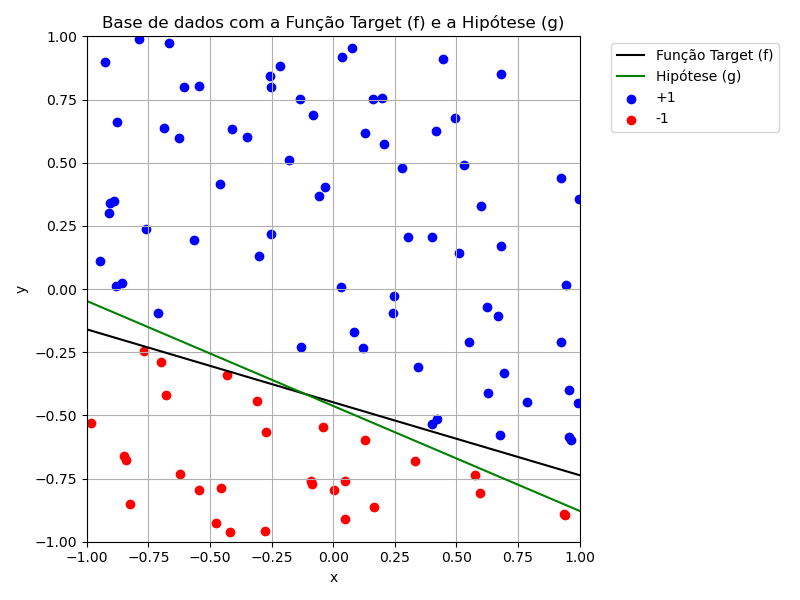
\includegraphics[width=12cm]{perceptron_plot.png}
    \label{fig:perceptron_plot}
\end{figure}

Pela figura \ref{fig:perceptron_plot}, é possível observar que a Hipótese (g) gera uma linha que, apesar de não sobrepor completamente a linha da Função Target (f), separa os pontos perfeitamente, resultado já esperado pelo treinamento utilizando o PLA, uma vez que esse algoritmo só converge quando o erro dentro da amosta $E_{in}$ é nulo.  

\begin{enumerate}
    \item Considere $N = 10$. Quantas iterações demora, em média, para que o PLA convirja com $N = 10$
    pontos de treinamento? Escolha o valor mais próximo do seu resultado.

    \begin{enumerate}
        \item[\textcolor{red}{(a)}]\textcolor{red}{1}\addtocounter{enumii}{1}
        \item 15
        \item 300
        \item 5000
        \item 10000
    \end{enumerate}
     
    \par

    \textbf{Justificativa:}

    Para responder a esse item foi implementada a seguinte função:

    \begin{lstlisting}[language=Python, caption=Cálculo do número de iterações, label=cod:perceptron_num_iter]
        def calc_num_iter(num_points, verbose = True):
        lista_iter = list()
        for _ in range(1000):
            target = Target()
            target.generate_random_line()
            dataset = Dataset(num_points)
            data, labels = dataset.generate_dataset(target)
            perceptron = Perceptron2D()
            iter, _ = perceptron.pla(data,labels)
            lista_iter.append(iter)
        if verbose: print(f"{np.mean(lista_iter)} iterações com desvio padrão {np.std(lista_iter):.4f} (min:{np.min(lista_iter)}, máx:{np.max(lista_iter)})")
        return lista_iter
    \end{lstlisting}

    O resultado após 1000 execuções do experimento, com a variável $num\_points = 10$, foi uma média de $5.0490(\approx 5)$ iterações, com desvio padrão de $7.7770(\approx 8)$ iterações, mínimo de 2 iterações e máximo de 99 iterações. Nota-se que o número de iterações pode variar bastante entre uma execução e outra, o que se deve ao alto grau de aleatoriedade presente no problema, uma vez que tanto os pontos quanto a reta da Função Target são gerados de forma aleatória, podendo levar a configurações de diferentes níveis de dificuldade para o PLA convergir. 
    % Apesar de toda essa aleatoriedade, em todas as execuções da função $calc\_num\_iter(num\_points)$ a média se manteve em torno de 5, tendo variando apenas o devio padrão.
     Como 5 está mais próximo de 1 do que de 15, o \textcolor{red}{\textbf{item a}} foi selecionado. 
    
    \item Qual das alternativas seguintes é mais próxima de $\mathbb{P}[f(x) \neq g(x)]$ para $N = 10$?
    
    \begin{enumerate}
        \item 0.001
        \item 0.01
        \item[\textcolor{red}{(c)}]\textcolor{red}{0.1}\addtocounter{enumii}{1}
        \item 0.5
        \item 1
    \end{enumerate}
     
    \par

    \textbf{Justificativa:}
     
    $\mathbb{P}[f(x) \neq g(x)]$ pode ser estimada computacionalmente gerando-se uma quiantidade suficientemente grande de pontos novos e calculando o percentual de erro na classificação desses pontos. Para responder esse item foram realizadas 1000 execuções, nas quais foram gerados 10010 pontos, sendo 10 utilizados para o treinamento do perceptron e 10 mil utilizados para teste. A cada execução foi calculado o perceltual de erro, isto é, a quantidade de vezes que a classificação do perceptron foi diferente da função target divido pela quantidade de pontos. No final das execuções, $\mathbb{P}[f(x) \neq g(x)]$ foi estimada fazendo a média do percentual de erro em cada execução. A Implementação pode ser vista abaixo:

    \begin{lstlisting}[language=Python, caption=Cálculo da probabilidade de erro, label=cod:perceptron_p_erro]
        def calc_p_erro(num_points, verbose = True):
        lista_erro = list()
        for _ in range(1000):
            target = Target()
            target.generate_random_line()
            dataset_train = Dataset(num_points)
            x_train, y_train = dataset_train.generate_dataset(target)
            dataset_test = Dataset(10000) # mais 10mil pontos
            x_test, y_test = dataset_test.generate_dataset(target)
            perceptron = Perceptron2D()
            perceptron.pla(x_train,y_train)
            y_predicted = perceptron.classificar(x_test)
            erro = np.mean(y_test != y_predicted)
            lista_erro.append(erro)
        if verbose: print(f"P[f(x)\u2260g(x)] = {np.mean(lista_erro):.4f}")
        return lista_erro
    \end{lstlisting}

    O resultado após 1000 execuções, com $num\_points = 10010$ e $train\_size = 10$, foi  $\mathbb{P}[f(x) \neq g(x)] = 0.0671 = 6.71\%$. Como 0.0671 está mais próximo de 0.1 do que de 0.01, o \textcolor{red}{\textbf{item c}} foi selecionado. 

    \item Agora considere $N = 100$. Quantas iterações demora, em média, para que o PLA convirja com
    N = 100 pontos de treinamento? Escolha o valor mais próximo do seu resultado.

    \begin{enumerate}
        \item[\textcolor{red}{(a)}]\textcolor{red}{50}\addtocounter{enumii}{1}
        \item 100
        \item 500
        \item 1000
        \item 5000
    \end{enumerate}
     
    \par

    \textbf{Justificativa:}

    Para responder a este item foi utilizada a mesma função do item 1 (código \ref{cod:perceptron_num_iter}), com $num\_points = 100$. 
    
    O resultado após 1000 execuções do experimento foi uma média de $32.981 (\approx 33)$ iterações, com desvio padrão de $164.5924 (\approx 165)$ iterações, mínimo de 2 iterações e máximo de 49 iterações. Nota-se que novamente o número de iterações pode variar bastante entre uma execução e outra, conforme já observado e explicado no item 1. Como 33 está abaixo de 50 e não existe alternativa menor, o \textcolor{red}{\textbf{item a}} foi selecionado. 
     

    \item Qual das alternativas seguintes é mais próxima de $\mathbb{P}[f(x) \neq g(x)]$ para $N = 100$?
    
    \begin{enumerate}
        \item 0.001
        \item[\textcolor{red}{(c)}]\textcolor{red}{0.01}\addtocounter{enumii}{1}
        \item 0.1
        \item 0.5
        \item 1
    \end{enumerate}

    \par

    \textbf{Justificativa:}

    Para responder a este item foi utilizada a mesma função do item 2 (código \ref{cod:perceptron_p_erro}), com $num\_points = 100$.

    O resultado após 1000 execuções foi  $\mathbb{P}[f(x) \neq g(x)] = 0.0069 = 0.69\%$. Como 0.0069 está mais próximo de 0.01 do que de 0.001, o \textcolor{red}{\textbf{item b}} foi selecionado. 
     
    
    \item  É possível estabelecer alguma regra para a relação entre $N$, o número de iterações até a convergência,
    e $\mathbb{P}[f(x) \neq g(x)]$?

    \par

    \textbf{Resposta:}

    Para responder a este item foram implementadas duas funções: uma para calcular o número de iterações e $\mathbb{P}[f(x) \neq g(x)]$ para uma faixa de diferentes números de pontos (código \ref{cod:perceptron_relationship}) e outra para plotar os resultados (código \ref{cod:perceptron_relationship_plot}). O código das duas pode ser observado abaixo.


    \begin{lstlisting}[language=Python, caption=Cálculo da probabilidade de erro e do número de iterações, label=cod:perceptron_relationship]
        def relationship(lista_num_points):
            lista_iter_medio = list()
            lista_erro_medio = list()
            for num_points in lista_num_points:
                lista_iter = calc_num_iter(num_points, verbose=False)
                lista_erro = calc_p_erro(num_points, verbose=False)
                lista_iter_medio.append(np.mean(lista_iter))  
                lista_erro_medio.append(np.mean(lista_erro))
            return lista_iter_medio, lista_erro_medio
    \end{lstlisting}

    \begin{lstlisting}[language=Python, caption=Plot da probabilidade de erro e do número de iterações, label=cod:perceptron_relationship_plot]
        def plot_relationship(num_points_list, lista_iter_medio, lista_erro_medio):
            fig, ax = plt.subplots(1, 1, figsize=(8, 8))
            ax.plot(num_points_list,lista_iter_medio,c="blue",label="Iterações")
            ax.set_title("Curvas de relação")
            ax.set_xlabel('Nº de pontos')
            ax.set_ylabel('Iterações')
            ax2=ax.twinx()
            ax2.plot(num_points_list,lista_erro_medio,c="red", label='P[f(x)\u2260g(x)]')
            ax2.set_ylabel('P[f(x)\u2260g(x)]')
            fig.legend(loc='upper center', bbox_to_anchor=(0.5, 0.9))
            fig.tight_layout()
            plt.show()
    \end{lstlisting}

    O resultado para o tamanho $N$ da amostra variando de 10 a 100 com passo 2 pode ser observado na figura \ref{fig:perceptron_relationship_plot}. 

    \begin{figure}[H]
        \caption{Resultado para $N$ variando de 10 a 100 com passo 2}
           \centering
           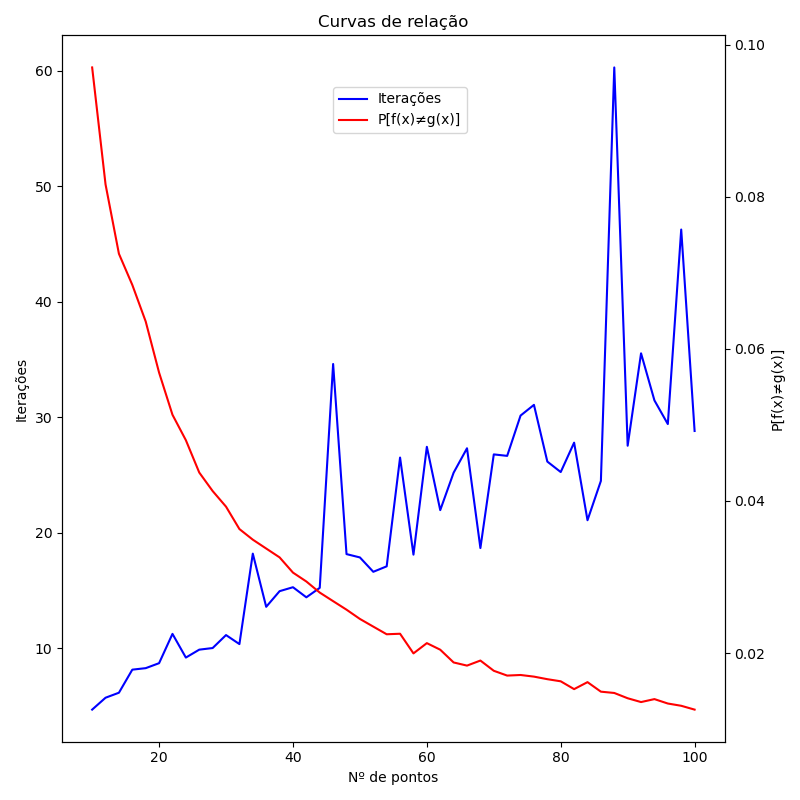
\includegraphics[width=12cm]{perceptron_relationship_plot.png}
        \label{fig:perceptron_relationship_plot}
    \end{figure}

    A quantidade de iterações para o PLA convergir, como constatado nos itens 1 e 3, oscila bastante, porém, pela figura, é possível observar que ela tem uma tendencia de alta conforme $N$ aumenta. Já a probabilidade de erro $\mathbb{P}[f(x) \neq g(x)]$ visivelmente apresenta uma queda exponencial com o aumento de $N$. Conclui-se que, com o aumento de $N$, o algoritmo se torna mais confiável, porém demora mais para ser treinado.
    
    
\end{enumerate}
\section{Regressão Linear}

Nestes problemas, nós vamos explorar como Regressão Linear pode ser usada em tarefas de classificação.
Você usará o mesmo esquema de produção de pontos visto na parte acima do Perceptron, com $d = 2$,
$\mathcal{X} = [-1, 1] \times [-1, 1]$, e assim por diante.

\begin{enumerate}
    \item Considere $N = 100$. Use Regressão Linear para encontrar $g$ e calcule $E_{in}$, a fração de pontos dentro da amostra que foram classificados incorretamente (armazene os $g$'s pois eles serão usados no item seguinte). Repita o experimento 1000 vezes. Qual dos valores abaixo é mais próximo do $E_{in}$ médio?
    
    \begin{enumerate}
        \item 0
        \item 0.001
        \item 0.01
        \item 0.1
        \item 0.5
        % [\textcolor{red}{(c)}]\textcolor{red}{0.01}\addtocounter{enumii}{1}
    \end{enumerate}

    \item Agora, gere 1000 pontos novos e use eles para estimar o $Eout$ dos $g$'s que você encontrou no item anterior. Novamente, realize 1000 execuções. Qual dos valores abaixo é mais próximo do $E_{out}$ médio?
    
    \begin{enumerate}
        \item 0
        \item 0.001
        \item 0.01
        \item 0.1
        \item 0.5
        % [\textcolor{red}{(c)}]\textcolor{red}{0.01}\addtocounter{enumii}{1}
    \end{enumerate}

    \item Agora, considere $N = 10$. Depois de encontrar os pesos usando Regressão Linear, use-os como um vetor de pesos iniciais para o Algoritmo de Aprendizagem Perceptron (PLA). Execute o PLA até que ele convirja num vetor final de pesos que separa perfeitamente os pontos dentro-de-amostra. Dentre as opções abaixo, qual é mais próxima do número médio de iterações (sobre 1000 execuções) que o PLA demora para convergir?
    
    \begin{enumerate}
        \item 1
        \item 15
        \item 300
        \item 5000
        \item 10000
        % [\textcolor{red}{(c)}]\textcolor{red}{0.01}\addtocounter{enumii}{1}
    \end{enumerate}
    
    \item Vamos agora avaliar o desempenho da versão pocket do PLA em um conjunto de dados que não é linearmente separável. Para criar este conjunto, gere uma base de treinamento com N2 pontos como foi feito até agora, mas selecione aleatoriamente 10\% dos pontos e inverta seus rótulos. Em seguida, implemente a versão pocket do PLA, treine-a neste conjunto não-linearmente separável, e avalie seu $E_{out}$ numa nova base de N2 pontos na qual você não aplicará nenhuma inversão de rótulos. Repita para 1000 execuções, e mostre o $E_{in}$ e $E_{out}$ médios para as seguintes configurações (não esqueça dos gráficos scatterplot, como anteriormente):
    
    \begin{enumerate}
        \item 0
        \item 0.001
        \item 0.01
        \item 0.1
        \item 0.5
        % [\textcolor{red}{(c)}]\textcolor{red}{0.01}\addtocounter{enumii}{1}
    \end{enumerate}

    
\end{enumerate}
\section{Regressão Não-Linear}

Nestes problemas, nós vamos novamente aplicar Regressão Linear para classificação. Considere a função target

$$f(x_1,x_2) = sign(x_1^2 + x_2^2 - 0.6) $$

Gere um conjunto de treinamento de $N = 1000$ pontos em $\mathcal{X} = [-1, 1] \times [-1, 1]$ com probabilidade uniforme escolhendo cada $x \in \mathcal{X}$. Gere um ruído simulado selecionando aleatoriamente 10\% do conjunto de treinamento e invertendo o rótulo dos pontos selecionados.

newline \par
\textbf{Implementação:}

Para responder os itens referentes a este problema, foram implementado em Python duas classes: uma para gerar a função target não-linear (código \ref{cod:target_naolin}) e outra para gerar o Classificador Não-Linear (código \ref{cod:reg_naolin}). 

\begin{lstlisting}[language=Python, caption=Target Não-Linear, label=cod:target_naolin]
    # Classe para criar a função target não linear
    class TargetNaoLinear:
    
        # Método para classificar pontos de acordo a função target
        def classify_point(self, point): 
            return np.sign(point[0]**2 + point[1]**2 - 0.6)
        
        # Método para criar uma elipse para plots
        def criar_elipse(self):
            r = np.sqrt(0.6)
            elipse =  Ellipse(xy=(0,0), width=2*r, height=2*r, angle=np.degrees(0),
                               edgecolor='k', fc='None', lw=2, label='Função Target (f)')
            return elipse
\end{lstlisting}

A classe para gerar a função target não-linear possui dois métodos: um para classificar os pontos de acordo com $f(x_1,x_2) = sign(x_1^2 + x_2^2 - 0.6) $ e outro que gera uma elipse a partir $f(x_1,x_2)$ para ser plotada. Esta classe poderia ter sido quebrada em duas funções, porém foi decidido criar uma classe para agrupar as duas funções e também para que ela continuasse funcionando como entrada para o método $generate\_dataset(target)$ da classe $Dataset$ (código \ref{cod:dataset}), reaproveitada neste problema para gerar a base de dados $\mathcal{X}$.

\begin{lstlisting}[language=Python, caption=Classificador por Regressão Não-Linear, label=cod:reg_naolin]
    # Classe para criar e treinar o classificador linear
    class NaoLinear(Linear):
        def __init__(self, w = np.zeros(6)):
            self.w = w  # inicializa os pesos (incluindo o w_0)
        
        # Modifica o método para calcular a matriz X
        def calc_matriz_X(self, data):
            X = list()
            for point in data:
                x1 = point[0]
                x2 = point[1]
                X.append([1, x1, x2, x1*x2, x1**2, x2**2])
            return np.array(X)
        
        # Método novo para criar uma elipse para plots
        def criar_elipse(self):
            # Coeficientes da equação geral da cônica (Ax1^2 + Bx1x2 + Cx2^2 + Dx1 + Ex2 + F=0)
            # relacionados com os pesos (1, x1, x2, x1x2, x1^2, x2^2)
            A = self.w[4] # coef de x1^2
            B = self.w[3] # coef de x1x2
            C = self.w[5] # coef de x2^2
            D = self.w[1] # coef de x1
            E = self.w[2] # coef de x2
            F = self.w[0] # termo independente
            # Matrizes associadas à equação geral da cônica
            M = np.array([[A, B / 2], [B / 2, C]])
            offset = np.array([D, E])
            # Calcular o centro da elipse
            center = np.linalg.solve(-2 * M, offset)
            # Calcular os semi-eixos e o ângulo de rotação
            eigenvalues, eigenvectors = np.linalg.eigh(M)
            order = np.argsort(eigenvalues)
            eigenvalues = eigenvalues[order]
            eigenvectors = eigenvectors[:, order]
            semi_major = np.sqrt(-F / (eigenvalues[0] * eigenvalues[1])) / np.sqrt(eigenvalues[0])
            semi_minor = np.sqrt(-F / (eigenvalues[0] * eigenvalues[1])) / np.sqrt(eigenvalues[1])
            angle = np.arctan2(eigenvectors[1, 0], eigenvectors[0, 0])
            # Criar a elipse
            elipse =  Ellipse(xy=center, width=2 * semi_major, height=2 * semi_minor, angle=np.degrees(angle),
                            edgecolor='g', fc='None', lw=2, label='Hipótese (g)')
            return elipse
\end{lstlisting}

A classe do Classificador Não-Linear herda a classe do Classificador Linear (código \ref{cod:reglin}), modifica a inicialização dos pesos e o método para gerar a matriz de entradas $X$ seguindo o vetor de atributos não-linear $(1, x_1, x_2, x_1x_2, x_1^2, x_2^2)$ e insere um novo método que gera uma elipse a partir pesos calculados (relacionando eles com a fórmula geral das cônicas) para ser plotada.

Para testar as classes foram criadas duas funções: uma para plotar o dataset não-linear juntamente com a função target e a hipotese (código \ref{cod:scatterplot_nao_linear}), e outra parar gerar os dados utilizando a função target não-linear e ainda gerando ruido em 10\% deles e depois treinar um Classificador Não-Linear (código \ref{cod:teste_nao_linear}).

\begin{lstlisting}[language=Python, caption=Scatterplot Não-Linear, label=cod:scatterplot_nao_linear]
    def scatterplot_nao_linear(data, labels, target, hipotese):
        fig, ax = plt.subplots(subplot_kw={'aspect': 'equal'}, figsize=(8, 6))
        # plotar a função target
        elipse_target = target.criar_elipse()
        ax.add_patch(elipse_target)
        # plotar a hipótese
        if type(hipotese) is NaoLinear:
            elipse_hipotese = hipotese.criar_elipse()
            ax.add_patch(elipse_hipotese)
        elif type(hipotese) is Linear:
            w = hipotese.w
            x = np.linspace(-1, 1, 100)
            y_g = -(w[1] * x + w[0]) / w[2]
            plt.plot(x, y_g, 'g-', label='Hipótese (g)')
        else:
            return print("Hipotese não suportada")
        # plotar os pontos
        x_pos = [data[i][0] for i in range(len(data)) if labels[i] == 1]
        y_pos = [data[i][1] for i in range(len(data)) if labels[i] == 1]
        x_neg = [data[i][0] for i in range(len(data)) if labels[i] == -1]
        y_neg = [data[i][1] for i in range(len(data)) if labels[i] == -1]
        plt.scatter(x_pos, y_pos, c='blue', label='+1')
        plt.scatter(x_neg, y_neg, c='red', label='-1')
        # ajustar a figura       
        plt.xlim(-1, 1)
        plt.ylim(-1, 1)
        plt.xlabel('x')
        plt.ylabel('y')
        plt.title('Base de dados com a Função Target (f) não linear e Hipótese (g)')
        plt.legend(bbox_to_anchor=(1.05, 1), loc='upper left')
        plt.tight_layout(rect=[0, 0, 1, 1])
        plt.grid(True)
        plt.show()
\end{lstlisting}

\begin{lstlisting}[language=Python, caption=Teste para a Regressão Não-Linear, label=cod:teste_nao_linear]
    def teste(num_points, hipotese):
        # Criar a target não-linear
        target = TargetNaoLinear()
        # Criar o dataset
        dataset = Dataset(num_points)
        data, labels = dataset.generate_dataset(target)
        # Adicionar ruido
        selected_indices = np.random.choice(len(labels), int(len(labels) * 0.1), replace=False) # seleciona 10%
        labels[selected_indices] *= -1 # inverte o valor de 10%
        # Criar o classificador
        hipotese.fit(data, labels)
        # Plotar
        scatterplot_nao_linear(data, labels, target, hipotese)
\end{lstlisting}

O resultado da função $teste(num\_points, hipotese)$ para uma hipótese gerada pelo treinamento de uma Regressão Não-Linear pode ser observado na figura \ref{fig:naolinear_naolinear}.

\begin{figure}[H]
    \caption{Base de dados com a Função Target $(f)$ Não-Linear e a Hipótese $(g)$ Não-Linear}
       \centering
       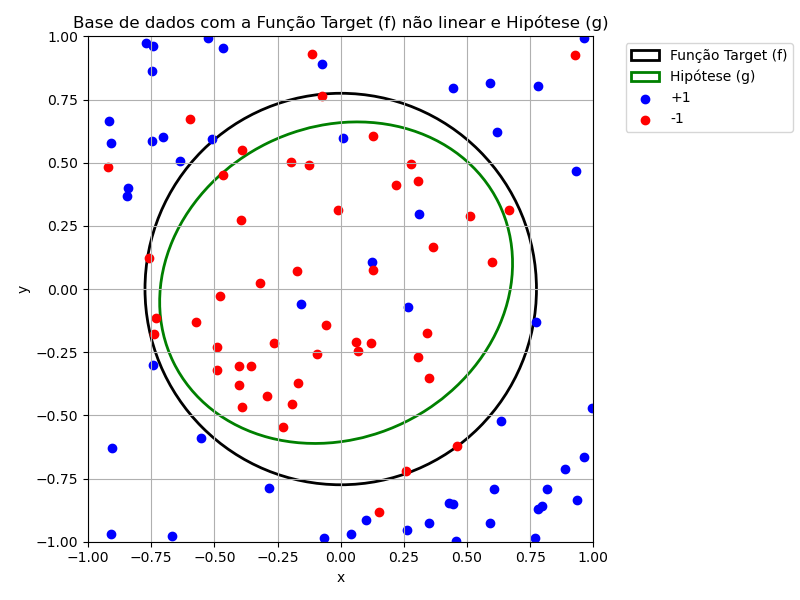
\includegraphics[width=12cm]{naolinear_naolinear.png}
       \label{fig:naolinear_naolinear}
\end{figure}

\begin{enumerate}
    \item Execute a Regressão Linear sem nenhuma transformação, usando o vetor de atributos $(1, x_1, x_2)$ para encontrar o peso $\boldsymbol{w}$. Qual é o valor aproximado de classificação do erro médio dentro da amostra $E_{in}$ (medido ao longo de 1000 execuções)?
    
    \begin{enumerate}
        \item 0
        \item 0.1
        \item 0.3
        \item [\textcolor{red}{(d)}]\textcolor{red}{0.5}\addtocounter{enumii}{1}
        \item 0.8
    \end{enumerate}
    
    \par

    \textbf{Justificativa:}

    Para responder a esse item foi implementada a seguinte função:

    \begin{lstlisting}[language=Python, caption=Cálculo do E\_in para a Regressão Linear, label=cod:calc_E_in_linear]
        def calc_Ein_linear(num_points, verbose = True):
            lista_E_in = list()
            for _ in range(1000):
                # Criar a target não-linear
                target = TargetNaoLinear()
                # Criar o dataset
                dataset = Dataset(num_points)
                data, labels = dataset.generate_dataset(target)
                # Adicionar ruido
                selected_indices = np.random.choice(len(labels), int(len(labels) * 0.1), replace=False) # seleciona 10%
                labels[selected_indices] *= -1 # inverte o valor de 10%
                # Criar o classificador não-linear
                linear = Linear()
                linear.fit(data, labels)
                # Classificar os pontos
                y_predicted = linear.classificar(data)
                # Calcular E_in para essa execução
                lista_E_in.append(np.mean(labels != y_predicted))
            E_in = np.mean(lista_E_in)
            # Plotar a última execução
            if verbose: print(f"E_in = {E_in:.4f}")
            return E_in
    \end{lstlisting}

    Foram realizadas 1000 execuções e em cada uma foi gerado um novo dataset para a função target $f(x_1,x_2) = sign(x_1^2 + x_2^2 - 0.6) $ e foi treinado um novo Classificador Linear. O $E_{in}$ em cada iteração foi calculado pelo número de erros dividido pela quantidade de pontos dentro da amostra. O valor final $E_{in} = 0.5044 = 50.44\%$ foi dado pela média dos $E_{in}$ em cada iteração. O valor de $E_{in}$ foi consideravelmente alto, como esperado de um Classificador Linear tentando classificar um dataset que não é linear. Como $0.5044$ está mais próximo de $0.5$ do que de $0.8$, o \textcolor{red}{item (d)} foi o escolhido.

    A figura \ref{fig:naolinear_linear} (gerada para apenas 100 pontos) ilustra por que o resultado do Regressor Linear foi tão ruim.

    \begin{figure}[H]
        \caption{Base de dados com a Função Target $(f)$ Não-Linear e a Hipótese $(g)$ Linear}
           \centering
           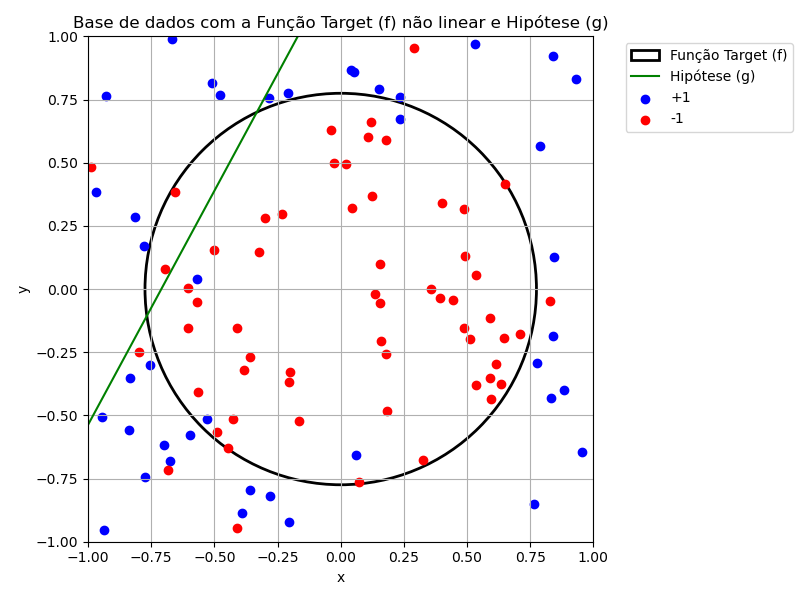
\includegraphics[width=12cm]{naolinear_linear.png}
           \label{fig:naolinear_linear}
    \end{figure}
    
    \item Agora, transforme os $N = 1000$ dados de treinamento seguindo o vetor de atributos não-linear $(1, x_1, x_2, x_1x_2, x_1^2, x_2^2)$. Encontre o vetor $\tilde{\boldsymbol{w}}$ que corresponda à solução da Regressão Linear. Quais das hipóteses a seguir é a mais próxima à que você encontrou? Avalie o resultado médio obtido após 1000 execuções.
    
    \begin{enumerate}
        \item [\textcolor{red}{(a)}]\textcolor{red}{$g(x_1,x_2) = sign(-1-0.05x_1+0.08x_2+0.13x_1x_2+1.5x_1^2+1.5x_2^2)$}\addtocounter{enumii}{1} 
        \item $g(x_1,x_2) = sign(-1-0.05x_1+0.08x_2+0.13x_1x_2+1.5x_1^2+15x_2^2)$
        \item $g(x_1,x_2) = sign(-1-0.05x_1+0.08x_2+0.13x_1x_2+15x_1^2+1.5x_2^2)$
        \item $g(x_1,x_2) = sign(-1-1.5x_1+0.08x_2+0.13x_1x_2+0.05x_1^2+0.05x_2^2)$
        \item $g(x_1,x_2) = sign(-1-0.05x_1+0.08x_2+1.5x_1x_2+0.15x_1^2+0.15x_2^2)$
    \end{enumerate}

    \par

    \textbf{Justificativa:}

    Para responder a esse item foi implementada a seguinte função:

    \begin{lstlisting}[language=Python, caption=Cálculo dos pesos para a Regressão Não-Linear, label=cod:calc_w_naolinear]
        def calc_w_naolinear(num_points, verbose = True):
            lista_w = list()
            for _ in range(1000):
                # Criar a target não-linear
                target = TargetNaoLinear()
                # Criar o dataset
                dataset = Dataset(num_points)
                data, labels = dataset.generate_dataset(target)
                # Adicionar ruido
                selected_indices = np.random.choice(len(labels), int(len(labels) * 0.1), replace=False) # seleciona 10%
                labels[selected_indices] *= -1 # inverte o valor de 10%
                # Criar o classificador não-linear
                naolinear = NaoLinear()
                w = naolinear.fit(data, labels)
                # Armazenar os pesos
                lista_w.append(w)
            w = np.mean(lista_w, axis=0)
            if verbose: 
                np.set_printoptions(suppress=True)
                print(f"w = {w}")
            return w
    \end{lstlisting}

    Foram realizadas 1000 execuções e em cada uma foi gerado um novo dataset para a função target $f(x_1,x_2) = sign(x_1^2 + x_2^2 - 0.6) $ e foi treinado um novo Classificador Não-Linear. O vetor $\boldsymbol{w}$ em cada iteração foi calculado pelo método $fit$ que multiplica a pseudo-inversa da matriz $X$ pelo vetor de labels. O valor final do vetor
     $$\tilde{\boldsymbol{w}} = [-0.9894, \quad -0.00164, \quad   0.0009, \quad   0.0031, \quad    1.5505, \quad   1.556]$$
      foi dado pela média em cada coluna da matriz $lista\_w$, a qual cada linha é composta pelo $\boldsymbol{w}$ calculado pelo treinamento naquela execução. O segundo, terceiro e quarto elementos divergem bastante das alternativas apresentadas, mas como o primeiro, o quinto e o sexto elementos se aproximam dos coeficientes da primeira alternativa, o \textcolor{red}{item (a)} foi o escolhido.
    
    \item Qual o valor mais próximo do erro de classificação fora da amostra $E_{out}$ de sua hipótese na questão anterior? (Estime-o gerando um novo conjunto de 1000 pontos e usando 1000 execuções diferentes, como antes).
    
    \begin{enumerate}
        \item [\textcolor{red}{(a)}]\textcolor{red}{0}\addtocounter{enumii}{1}
        \item 0.1 *
        \item 0.3
        \item 0.5
        \item 0.8
    \end{enumerate}

    Para responder a esse item foi implementada a seguinte função:

    \begin{lstlisting}[language=Python, caption=Cálculo do E\_out para a Regressão Não-Linear, label=cod:calc_E_out_naolinear]
        def calc_Eout_naolinear(num_points, w, verbose = True):
            lista_E_out = list()
            for _ in range(1000):
                # Criar a target não-linear
                target = TargetNaoLinear()
                # Criar o dataset de teste
                dataset = Dataset(num_points)
                data, labels = dataset.generate_dataset(target)
                # Criar o classificador não-linear
                naolinear = NaoLinear(w = w) # força a usar os pesos anteriores
                # Classificar os pontos com a mesma hipotese do E_in
                y_predicted = naolinear.classificar(data)
                # Calcular E_out para essa execução
                lista_E_out.append(np.mean(labels != y_predicted))
            E_out = np.mean(lista_E_out)
            if verbose: print(f"E_out = {E_out:.4f}")
            return E_out
    \end{lstlisting}

    Foram realizadas 1000 execuções e em cada uma foi gerado um novo dataset para a função target $f(x_1,x_2) = sign(x_1^2 + x_2^2 - 0.6) $ e Classificador Linear foi gerado reutilizando o $\tilde{\boldsymbol{w}}$ calculado no item anterior. O $E_{out}$ em cada iteração foi calculado pelo número de erros dividido pela quantidade de pontos dentro da amostra. O valor final $E_{out} = 0.0291 = 2.91\%$ foi dado pela média dos $E_{out}$ em cada iteração. Como $0.0291$ está mais próximo de $0$ do que de $0.1$, o \textcolor{red}{item (a)} foi o escolhido.

\end{enumerate}






\end{document}